% 图 6.14（按原书 124 页样式：公式式排版 |Φ⟩=⋯↑↑↑⋯，无格点圆圈）
% 态 |Φ⟩ 全部沿 +z；态 |j⟩ 在格点 j 处一个自旋翻转
\documentclass[tikz,border=5pt]{standalone}
\usetikzlibrary{arrows.meta}
\usepackage{amsmath}
\usepackage{bm}
\usepackage{fontspec}
\setmainfont{Times New Roman}
\begin{document}
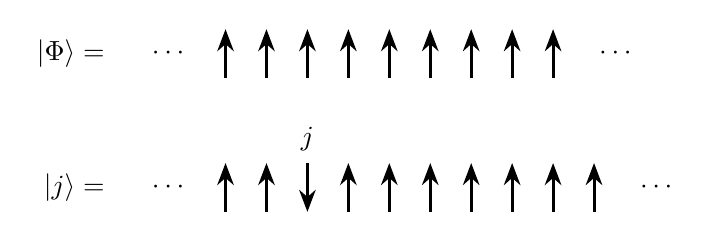
\begin{tikzpicture}[>=Stealth,line width=1.1pt]
\def\dx{0.52}
% ---- |Φ⟩ = ⋯ 9 个向上箭头 ⋯ ----
\node[anchor=east] at (-0.35,0.41) {$|\Phi\rangle = $};
\node at (0.35,0.41) {$\cdots$};
\foreach \i in {0,...,8}{
  \draw[->] ({1.05+\i*\dx},0.10) -- ({1.05+\i*\dx},0.72);}
\node at ({1.05+9*\dx+0.3},0.41) {$\cdots$};
% ---- |j⟩ = ⋯ ↑↑↓↑↑↑↑↑↑↑ ⋯，j 标在翻转的自旋上方 ----
\begin{scope}[shift={(0,-1.7)}]
\node[anchor=east] at (-0.35,0.41) {$|j\rangle = $};
\node at (0.35,0.41) {$\cdots$};
\draw[->] ({1.05+0*\dx},0.10) -- ({1.05+0*\dx},0.72);
\draw[->] ({1.05+1*\dx},0.10) -- ({1.05+1*\dx},0.72);
\draw[->] ({1.05+2*\dx},0.72) -- ({1.05+2*\dx},0.10);   % 翻转的自旋
\node at ({1.05+2*\dx},1.02) {$j$};
\foreach \i in {3,...,9}{
  \draw[->] ({1.05+\i*\dx},0.10) -- ({1.05+\i*\dx},0.72);}
\node at ({1.05+10*\dx+0.3},0.41) {$\cdots$};
\end{scope}
\end{tikzpicture}
\end{document}
